\documentclass[a4paper,12pt,twoside]{memoir}

% Castellano
\usepackage[spanish,es-tabla]{babel}
\selectlanguage{spanish}
\usepackage[utf8]{inputenc}
\usepackage[T1]{fontenc}
\usepackage{lmodern} % Scalable font
\usepackage{microtype}
\usepackage{placeins}

\RequirePackage{booktabs}
\RequirePackage[table]{xcolor}
\RequirePackage{xtab}
\RequirePackage{multirow}

% Links
\PassOptionsToPackage{hyphens}{url}\usepackage[colorlinks]{hyperref}
\hypersetup{
	allcolors = {red}
}

% Ecuaciones
\usepackage{amsmath}

% Rutas de fichero / paquete
\newcommand{\ruta}[1]{{\sffamily #1}}

% Párrafos
\nonzeroparskip

% Huérfanas y viudas
\widowpenalty100000
\clubpenalty100000

\let\tmp\oddsidemargin
\let\oddsidemargin\evensidemargin
\let\evensidemargin\tmp
\reversemarginpar

% Imágenes

% Comando para insertar una imagen en un lugar concreto.
% Los parámetros son:
% 1 --> Ruta absoluta/relativa de la figura
% 2 --> Texto a pie de figura
% 3 --> Tamaño en tanto por uno relativo al ancho de página
\usepackage{graphicx}

\newcommand{\imagen}[3]{
	\begin{figure}[!h]
		\centering
		\includegraphics[width=#3\textwidth]{#1}
		\caption{#2}\label{fig:#1}
	\end{figure}
	\FloatBarrier
}







\graphicspath{ {./img/} }

% Capítulos
\chapterstyle{bianchi}
\newcommand{\capitulo}[2]{
	\setcounter{chapter}{#1}
	\setcounter{section}{0}
	\setcounter{figure}{0}
	\setcounter{table}{0}
	\chapter*{#2}
	\addcontentsline{toc}{chapter}{#2}
	\markboth{#2}{#2}
}

% Apéndices
\renewcommand{\appendixname}{Apéndice}
\renewcommand*\cftappendixname{\appendixname}

\newcommand{\apendice}[1]{
	%\renewcommand{\thechapter}{A}
	\chapter{#1}
}

\renewcommand*\cftappendixname{\appendixname\ }

% Formato de portada

\makeatletter
\usepackage{xcolor}
\newcommand{\tutor}[1]{\def\@tutor{#1}}
%\newcommand{\tutorb}[1]{\def\@tutorb{#1}}

\newcommand{\course}[1]{\def\@course{#1}}
\definecolor{cpardoBox}{HTML}{E6E6FF}
\def\maketitle{
  \null
  \thispagestyle{empty}
  % Cabecera ----------------
\begin{center}
  \noindent
\includegraphics[width=\textwidth]{cabeceraSalud}\vspace{1.5cm}%
\end{center}
  
  % Título proyecto y escudo salud ----------------
  \begin{center}
    \begin{minipage}[c][1.5cm][c]{.20\textwidth}
        
\includegraphics[width=\textwidth]{escudoSalud.pdf}
    \end{minipage}
  \end{center}
  
  \begin{center}
    \colorbox{cpardoBox}{%
        \begin{minipage}{.8\textwidth}
          \vspace{.5cm}\Large
          \begin{center}
          \textbf{TFG del Grado en Ingeniería de la Salud}\vspace{.6cm}\\
          \textbf{\LARGE\@title{}}
          \end{center}
          \vspace{.2cm}
        \end{minipage}
    }%
  \end{center}
  
    % Datos de alumno, curso y tutores ------------------
  \begin{center}%
  {%
    \noindent\LARGE
    Presentado por \@author{}\\ 
    en Universidad de Burgos\\
    \vspace{0.5cm}
    \noindent\Large
    \@date{}\\
    \vspace{0.5cm}
    Tutor: \@tutor{}\\ 
    %Tutores: \@tutor{} -- \@tutorb{}\\
  }%
  \end{center}%
  \null
  \cleardoublepage
  }
\makeatother
\newcommand{\nombre}{Claudia Valentín Alguacil}
\newcommand{\nombreTutor}{Pedro Luis Sanchez Ortega} 
%\newcommand{\nombreTutorb}{Tutor 2} 
\newcommand{\dni}{03951611G} 

% Datos de portada
\title{Seguimiento clínico de pacientes con afectaciones en la mano con la ayuda de sensores de fuerza}
\author{\nombre}
\tutor{\nombreTutor}
\date{\today}

\begin{document}

\maketitle


\newpage\null\thispagestyle{empty}\newpage

%%%%%%%%%%%%%%%%%%%%%%%%%%%%%%%%%%%%%%%%%%%%%%%%%%%%%%%%%%%%%%%%%%%%%%%%%%%%%%%%%%%%%%%%
\thispagestyle{empty}


\noindent
\includegraphics[width=\textwidth]{cabeceraSalud}\vspace{1cm}

\noindent D. \nombreTutor, profesor del departamento de Ingeniería Electromecánica, área Tecnología Electrónica.

\noindent Expone:

\noindent Que la alumna Dª. \nombre, con DNI \dni, ha realizado el Trabajo final de Grado en Ingeniería de la Salud titulado Seguimiento clínico de pacientes con afectaciones en la mano con la ayuda de sensores de fuerza. 

\noindent Y que dicho trabajo ha sido realizado por el alumno bajo la dirección del que suscribe, en virtud de lo cual se autoriza su presentación y defensa.

\begin{center} %\large
En Burgos, {\large \today}
\end{center}

\vfill\vfill\vfill

% Author and supervisor
\begin{minipage}{0.45\textwidth}
\begin{flushleft} %\large
Vº. Bº. del Tutor:\\[2cm]
D. \nombreTutor
\end{flushleft}
\end{minipage}
\hfill
\begin{minipage}{0.45\textwidth}
\begin{flushleft} %\large
%Vº. Bº. del Tutor:\\[2cm]
%D. \nombreTutorb
\end{flushleft}
\end{minipage}
\hfill

\vfill

% para casos con solo un tutor comentar lo anterior
% y descomentar lo siguiente
%Vº. Bº. del Tutor:\\[2cm]
%D. nombre tutor


\newpage\null\thispagestyle{empty}\newpage




\frontmatter

% Abstract en castellano
\renewcommand*\abstractname{Resumen}
\begin{abstract}
Este proyecto se centra en la búsqueda de resolver un problema real, creando un prototipo de dispositivo e interfaz para cuantificar la fuerza que los pacientes pueden ejercer en las sesiones de terapia y establecer un registro a lo largo del tiempo de estas.

A pesar de que estos tipos de dispositivos ya existen, los hospitales públicos no están dotados de ellos debido a su alto precio y los escasos recursos en algunas áreas de los hospitales. La iniciativa de la creación de este proyecto, surge como respuesta a la necesidad comentada desde el área de terapia ocupacional. 

Se han estudiado los dispositivos que ya están en el mercado, para posteriormente realizar una búsqueda de los componentes más idóneos para el dispositivo a crear. Se ha creado un prototipo físico con sensores de fuerza resistivos y una interfaz básica para la visualización y registro de las cuantificaciones de fuerza.
\end{abstract}

\renewcommand*\abstractname{Descriptores}
\begin{abstract}
Sensor de Fuerza Resistivo, terapia ocupacional, cuantificación, fuerza, dinamómetro , mano, Arduino, bajo coste.
\ldots
\end{abstract}

\clearpage

% Abstract en inglés
\renewcommand*\abstractname{Abstract}
\begin{abstract}
This project focuses on searching for a real issue by creating a prototype device and interface to quantify the strength that patients can apply during therapy sessions, and to establish a record of these measurements over time.

Despite similar devices already existing, many public hospitals often are not equipped with them due to their high cost and the limited resources available in some certain hospital departments. 
The initiative for this project arose in response to an actual need expressed by the occupational therapy department.

Research has been conducted on the devices currently available on the market, followed by an investigation on potential components that could be used to build a new device. A physical prototype has been developed using force sensing resistors, along with a basic interface for visualizing and recording the strength measurements.
\end{abstract}

\renewcommand*\abstractname{Keywords}
\begin{abstract}
Force sensing resistors, occupational therapy, quantification, strength, hand, dinamometer, Arduino, low cost.
\end{abstract}

\clearpage

% Indices
\tableofcontents

\clearpage

\listoffigures

\clearpage

\listoftables
\clearpage


\mainmatter
\capitulo{1}{Introducción}
Este proyecto tuvo su origen durante las prácticas curriculares que realicé en diversas áreas del Hospital Universitario de Burgos, en particular en el área de Terapia Ocupacional. 

Las terapeutas ocupacionales me dieron a conocer su trabajo, incluso en algunas ocasiones haciéndome partícipe de ello. Durante este proceso pude observar su forma de trabajar, los recursos que tienen y las diferentes dificultades que enfrentan en su día a día, tanto por falta de recursos como por la falta de implementación tecnológica que les permitiría tanto optimizar los tratamientos como mejorar en el seguimiento de estos mismos.

Una de las muchas necesidades que me comunicaron fue la de tener un dispositivo capaz de medir la presión ejercida por un paciente con la mano al realizar ejercicios con la tabla canadiense. De tal manera que el dispositivo permitiría visualizar el valor de presión en el momento, sino también poder realizar un registro pudieran tener un registro de estas mediciones para poder observar la evolución o no evolución de un paciente y/o ver el momento de la sesión en el que el paciente se fatiga.

No está pensado para enfocarse en una única patología de la mano, sino que pretende ser útil tanto para el tratamiento como para el seguimiento de diferentes patologías de la mano.

La presente memoria del proyecto está estructurada en 7 capítulos, organizados especialmente para que faciliten su comprensión.
\begin{itemize}
    \item \textbf{Capítulo 1}: Descripción del contenido del proyecto,estructura de la memoria y materiales utilizados.
    \item \textbf{Capítulo 2}: Objetivos principales del proyecto y personales.
    \item \textbf{Capítulo 3}:Descripción de conceptos teóricos y estado del arte.
    \item \textbf{Capítulo 4}:Descripción de técnicas y herramientas utilizadas
    \item \textbf{Capítulo 5}:Resumen de resultados 
    \item \textbf{Capítulo 6}:Conclusiones 
    \item \textbf{Capítulo 7}:Posibles lineas futuras que pueda tener el proyecto
\end{itemize}
\include{./tex/2_objetivos}
\capitulo{3}{Conceptos teóricos}
\section{Conceptos teóricos básicos}
Para facilitar la comprensión del proyecto, he seleccionado una serie de conceptos útiles a definir. 
\begin{itemize}
    \item Dinamómetro: artefacto destinado a la medición de la fuerza y el peso de los objetos a partir de la elasticidad de un resorte o muelle elástico.\cite{Dinamometro}
    \item Terapia ocupacional: una profesión socio-sanitaria que se enfoca en ayudar a las personas a desarrollar, recuperar o mantener la capacidad para realizar actividades cotidianas y ocupaciones significativas. \cite{T.O}\footnote{Página web con información sobre la terapia ocupacional\cite{T.O}.}
    \item Transductor: dispositivo al que se aplica una energía de entrada y devuelve una energía de salida.\cite{celulas_extensométricas}
    \item Relación lineal: conexión entre dos variables que puede representarse gráficamente como una línea recta. En términos estadísticos, esta relación implica que cuando una variable cambia, la otra variable cambia de manera consistente.\cite{LEARN_STATISTICS_EASILY}
    \item Fatiga Muscular: es la incapacidad para seguir generando un nivel de fuerza o una intensidad de ejercicio determinada. \cite{gomez_campos_mecanismos_2010}
    \item Sensor de Fuerza Resistivo (FSR): son sensores capaces de detectar la presión o fuerza que se les ejerce. Como su propio nombre dice, necesita para su uso una resistencia, la cual actúa como divisor de voltaje
    \item Tabla canadiense: instrumento de mecanoterapia que se utiliza en el tratamiento y rehabilitación de lesiones de la mano.\ref{fig:tabla canadiense}\cite{cantero_tellez_terapia_2020}
    \begin{figure}
        \centering
        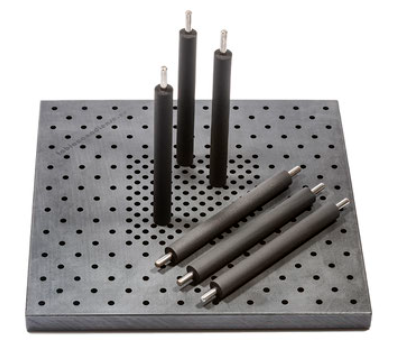
\includegraphics[width=0.5\linewidth]{img/Tabla_Canadiense.png}
        \caption{Tabla canadiense. Fuente tablacanadiense.es}
        \label{fig:tabla canadiense}
    \end{figure}

\section{Estado del arte.}

El proyecto ha de comenzar con búsqueda en el panorama actual en la medida de fuerza. 

En esta subsección se analiza y sintetiza el conocimiento existente en el área específica del proyecto. El objetivo principal es situar el trabajo dentro de un marco teórico y tecnológico, analizando investigaciones previas, aportes y detectando problemas que se puedan resolver.
\subsection{Dinamómetros:}
En la actualidad, los dinamómetros son una de las herramientas más utilizadas  para la medida de fuerza de los pacientes durante las sesiones de terapia ocupacional, fisioterapia o medicina deportiva. Existen diferentes modelos en el mercado que se diferencian en precisión, tecnología, precio o aplicación. 
A continuación, he destacado algunos de ellos:
\begin{itemize}
    \item Activforce 2: Es un dispositivo portátil e inalámbrico creado por la empresa estadounidense Activforce, con sede en California. Combina un dinamómetro con un inclinómetro lo que permite medir la fuerza máxima,promedio, rango de movimiento y simetría derecha-izquierda tanto en fuerza como en movimiento.Todas las mediciones se registran en una aplicación compatible con Android e iOS, donde el usuario puede ver toda la información recabada por el dispositivo.\cite{activforce}\footnote{Página web del dinamómetro Activforce2 con la información general del producto \cite{activforce}.}
    
    En la \textit{Figura} \ref{fig:activforce} se puede ver una imagen del producto.
    \begin{figure}[h]
        \centering
        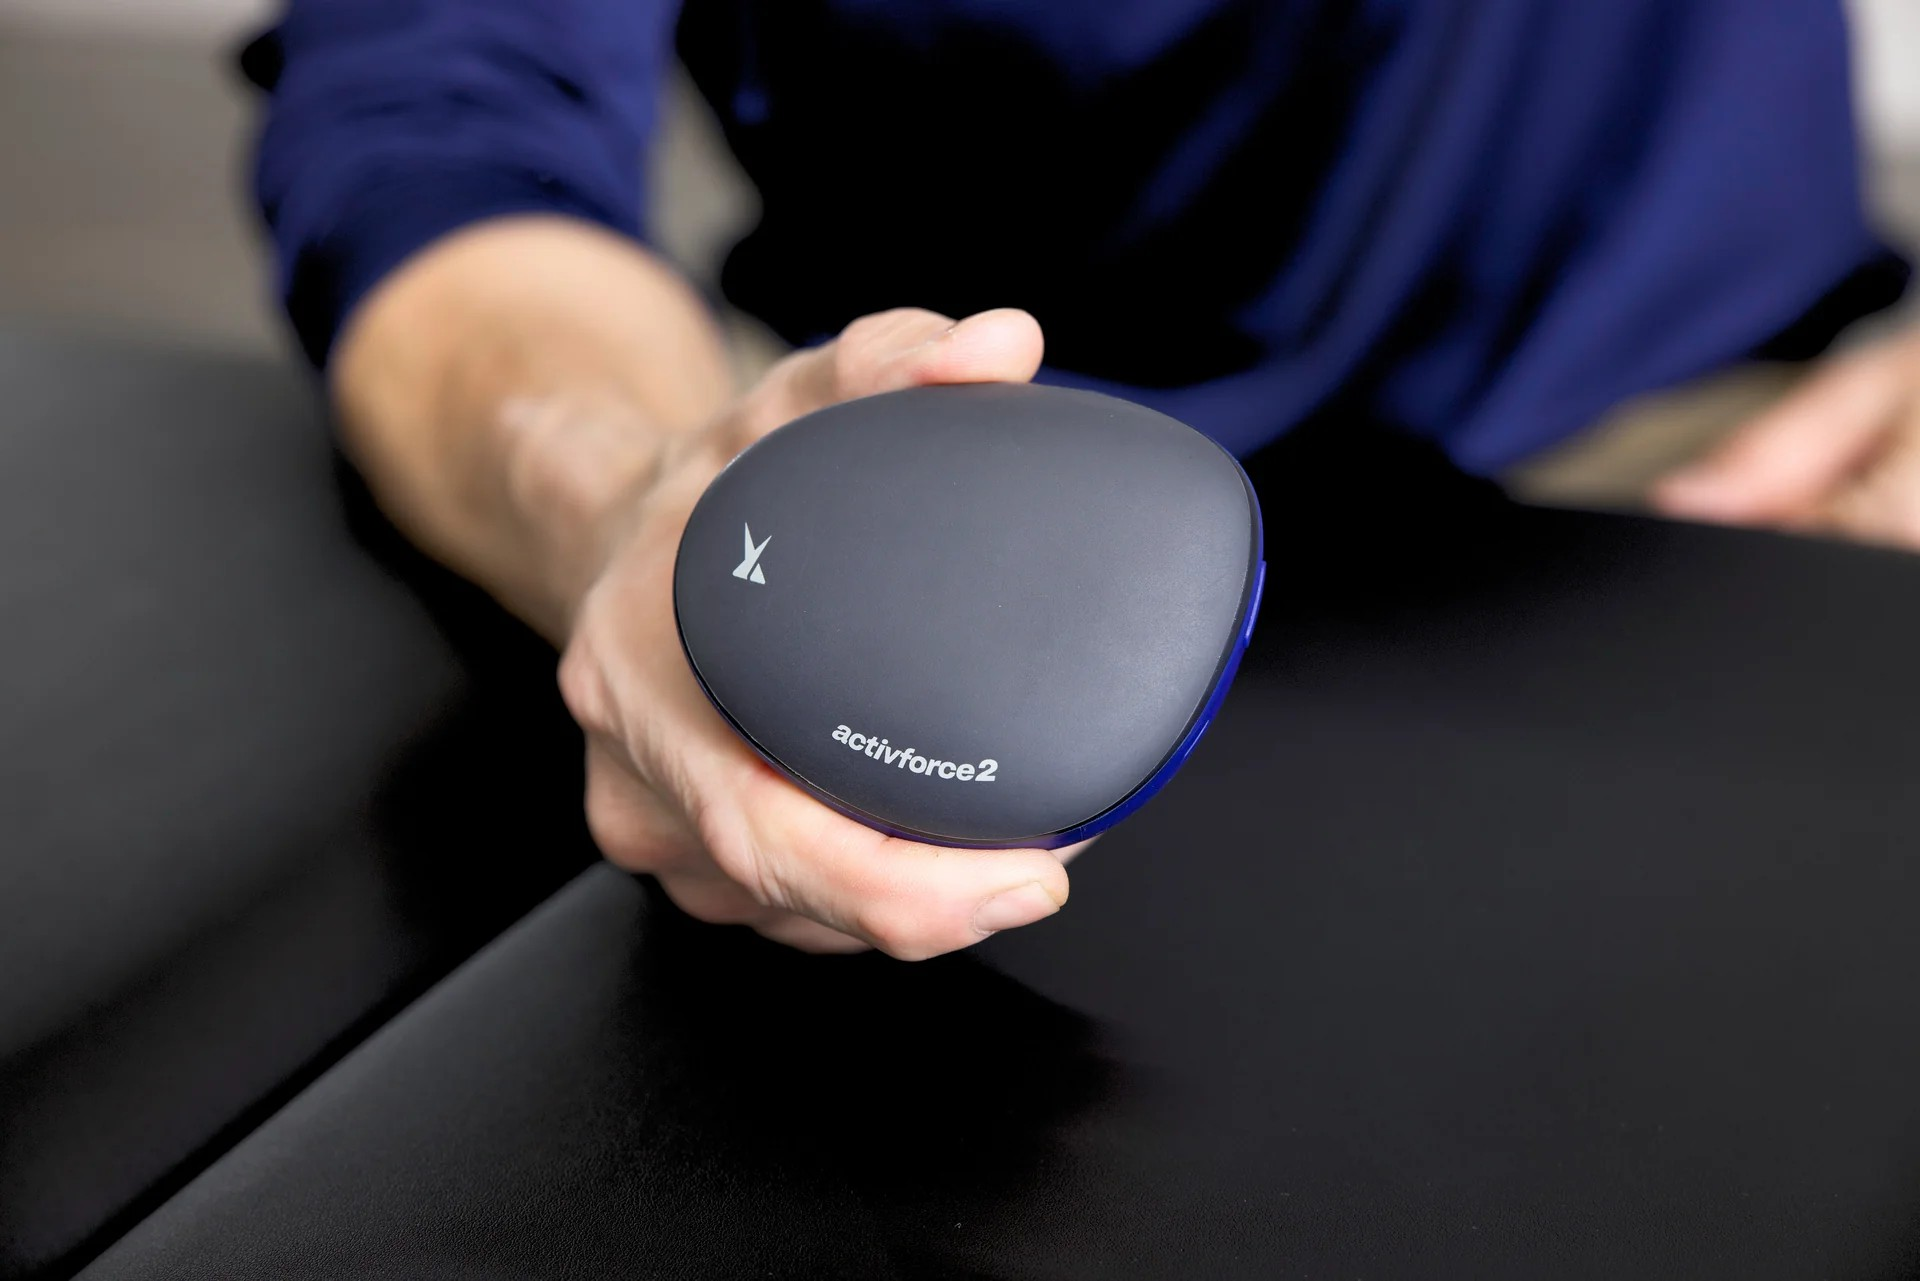
\includegraphics[width=0.5\textwidth]{img/ActivForce_Device.jpg}
        \caption{Dispositivo ActivForce2. Fuente activforce.com}
        \label{fig:activforce}
    \end{figure}
    
    Además, el Activforce 2 incluye varios accesorios que facilitan su uso en diferentes partes del cuerpo, permitiendo la ejecución de una amplia variedad de ejercicios y evaluaciones. Es un dispositivo de compra libre cuyo precio ronda los 450€. En la \textit{Figura} \ref{fig:activforce_Attachments} se puede ver una imagen del producto y los accesorios.
    \begin{figure}[h]
        \centering
        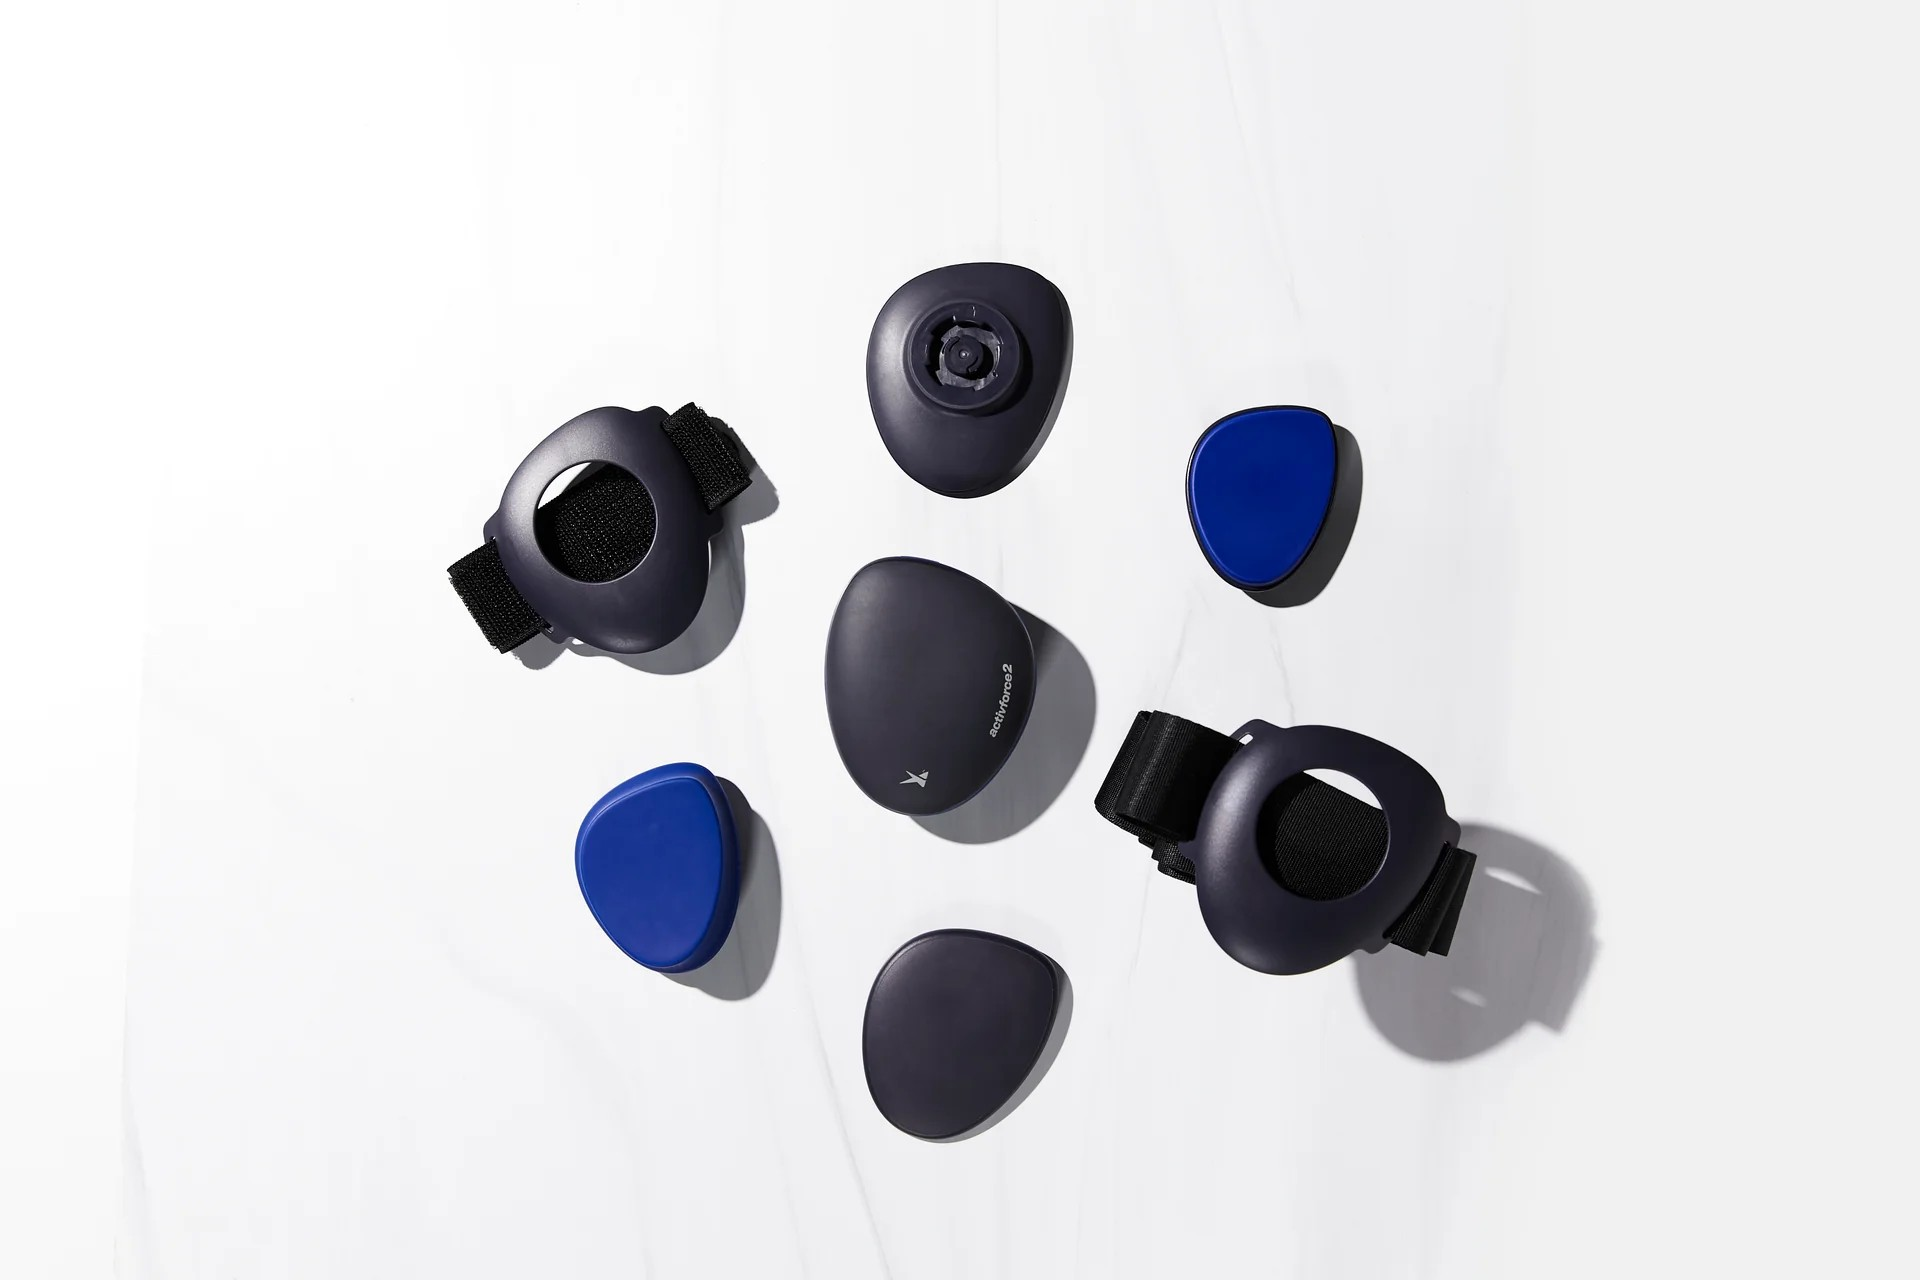
\includegraphics[width=0.5\textwidth]{img/ActivForce_Attachments.jpg}
        \caption{Accesorios compatibles con el dispositivo ActivForce2. Fuente activforce.com}
        \label{fig:activforce_Attachments}
    \end{figure}

    \item MicroFET 2: Es un dispositivo portátil e inalámbrico creado por la empresa belga MVS in motion. Es un dinamómetro diseñado para la evaluación y prueba de fuerza permite tomar mediciones de prueba muscular objetivas, cuantificables y confiables. 
    Es utilizado para la ayuda en el diagnóstico, pronóstico y el tratamiento de trastornos musculares. Presenta una pantalla digital donde se puede observar el valor de las mediciones en tiempo real. \cite{microfet}\footnote{Página web del dinamómetro MicroFET2 con la información general del producto \cite{microfet}.}
    Es un dispositivo de compra libre cuyo precio ronda los 1200€. 
    
    En la \textit{Figura} \ref{fig:MicroFET 2} se puede ver una imagen del dispositivo.
    \begin{figure}[h]
        \centering
        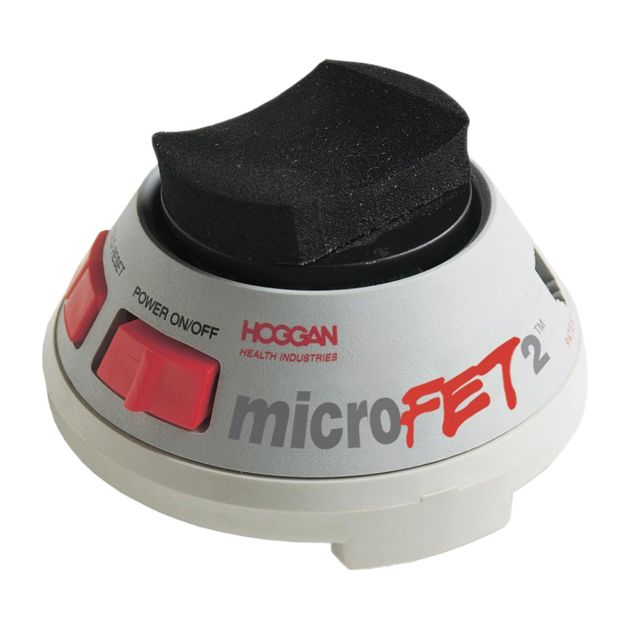
\includegraphics[width=0.45\textwidth]{img/MicroFET 2.jpg}
        \caption{Dispositivo MicroFET 2. Fuente fysiosupplies.es}
        \label{fig:MicroFET 2}
    \end{figure}
    
    \item MAP 80K1S: Es un dispositivo portátil e inalámbrico creado por la empresa alemana KERN \& SOHN. Es un dinamómetro de mano utilizado específicamente para tratamientos de rehabilitación, para la determinación de la fuerza de cierre de mano.
    Presenta cuatro modos de medición: tiempo real, valor máximo. valor promedio y de contaje. 
    Es utilizado en sesiones de rehabilitación para detectar la disminución de fuerza y la evolución del paciente entre sesiones. Cuenta con una pantalla digital donde se puede observar las mediciones realizadas. 
    Es un dispositivo de compra libre cuyo precio ronda los 280€. \cite{Map80k1s}\footnote{Página web del dinamómetro Map80K1S con la información general del producto \cite{Map80k1s}.}
    
    En la \textit{Figura} \ref{fig:Dispositivo MAP 80K1S} se puede ver una imagen del dispositivo.
      \begin{figure}[h]
        \centering
        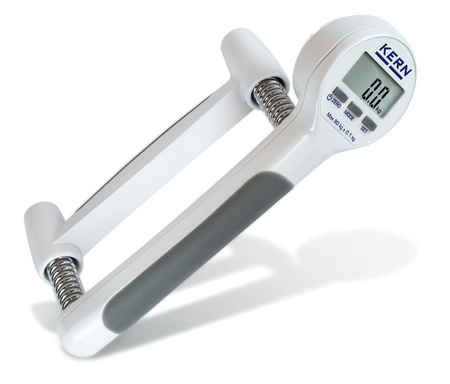
\includegraphics[width=0.5\textwidth]{img/MAP-80K1S.jpg}
        \caption{Dispositivo MAP 80K1S. Fuente kern-sohn.com}
        \label{fig:Dispositivo MAP 80K1S}
    \end{figure}
    
    \item Squeezy dynamometer: Es un dispositivo portátil, un dinamómetro de presión hidráulica de mano cuya medición se realiza apretando la perilla, generando presión que se transfiere al calibrador, el cual muestra con precisión la fuerza ejercida. Es un dispositivo de compra libre cuyo precio ronda los 70 €. \cite{SqueezeDinamometro}\footnote{Página web del dinamómetro Squeezy con la información general del producto \cite{SqueezeDinamometro}.} 
    
    En la \textit{Figura \ref{fig:Dinamómetro de Pera}} se puede ver una imagen del dispositivo.
    \begin{figure}[h]
        \centering
        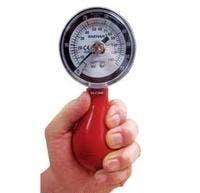
\includegraphics[width=0.5\textwidth]{img/Dinamometro pera.jpeg}
        \caption{Dinamómetro de Pera. Fuente rehabmedic.com}
        \label{fig:Dinamómetro de Pera}
    \end{figure}
\end{itemize}
\subsection{Artículos relacionados:}
La cuantificación de la fuerza en las manos  y su posterior análisis, es un tema que ya ha sido tratado por otros equipos de investigación en varios países. 

En esta subsección presentaré los artículos que he encontrado relacionados con el área, abarcando tanto la creación de dispositivos para la medición de la fuerza como el uso de dinamómetros para el registro de la evolución de los pacientes.
\begin{itemize}
    \item \textbf{Dispositivo de medición de fuerza de los dedos y su
rol en el seguimiento de las funciones de la mano}

Juliana Gomez et al, en su artículo llamado 'Dispositivo de medición de fuerza de los dedos y su rol en el seguimiento de las funciones de la mano' publicado en la revista de cirugía plástica Ibero Latinoamericana aborda la creación de un dispositivo capaz de medir la fuerza de los dedos de manera individual, para su uso en la evaluación del paciente sano y de pacientes con patologías traumáticas y no traumáticas, para determinar grados de discapacidad, seguimiento de enfermedades y/o recuperaciones. 
Este dispositivo se basa en el uso de 5 sensores del tipo Flexiforce A301 de la empresa TESKA®, sistema embebido
tipo Arduino y Matlab, se puede observar en la \textit{Figura \ref{fig:Dinamómetro creado por Juliana Gomez}}. Además, afirman la validez de su uso tras realizar un estudio con veinte sujetos sanos, obteniendo tasas de medición equiparables a las de otros sistemas.\cite{GOMEZ2022}\footnote{Artículo de la creación de un dispositivo con sensores de fuerza\cite{GOMEZ2022}.}
    \begin{figure}[h]
        \centering
        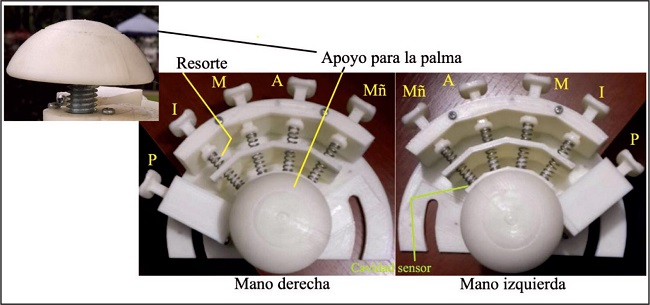
\includegraphics[width=0.7\textwidth]{img/dispositivo Revista.jpg}
        \caption{Dinamómetro creado por Juliana Gomez. Fuente scielo.isciii.es}
        \label{fig:Dinamómetro creado por Juliana Gomez}
    \end{figure}
\item \textbf{Uso del dinamómetro para mejorar la fuerza de la mano del adulto mayor.}
    
Mayra Lasteña Millingalli Ortega et al, en su artículo de revisión llamado 'Uso del dinamómetro para mejorar la fuerza de la mano del adulto mayor' publicado en la Revista Científica Arbitrada Multidisciplinaria PENTACIENCIAS en Octubre de 2023, realizan un trabajo de investigación revisando artículos en inglés y español publicados entre 2013 y 2022.
La población de estudio son pacientes geriátricos tratados en Terapia Ocupacional, las investigadoras exponen que actualmente en estas sesiones de terapia los pacientes son evaluados mediante métodos manuales como las escalas de registros, afirman que estos métodos son rudimentarios y no evidentes. \cite{Articulo_din}\footnote{Artículo que habla sobre el uso del dinamómetro\cite{Articulo_din}.}
\item \textbf{Diseño de dinamómetro con enfoque al monitoreo de fuerza de agarre de mano, en la 'Clínica Niño Sano' de niños quemados.}

    Tesis realizada en la universidad de Guatemala por Luis Carlos Ralon Gordillo en 2019, alumno del grado de  Ingeniería Mecatrónica. 

    Su tesis se fundamenta en la creación de un dispositivo para el monitoreo de la recuperación de la fuerza motriz de niños con quemaduras de tercer grado en la mano, utilizando un sensor de fuerza resistiva y un  microcontrolador PIC 16F88.

    En la \textit{Figura} \ref{fig:Prototipo dinamómetro Luis} se puede observar el prototipo realizado por el alumno.

    En el Luis Carlos Ralon afirma el correcto funcionamiento de su dispositivo, teniendo el sensor un  error promedio de 5.50 \%.

    \begin{figure}
        \centering
        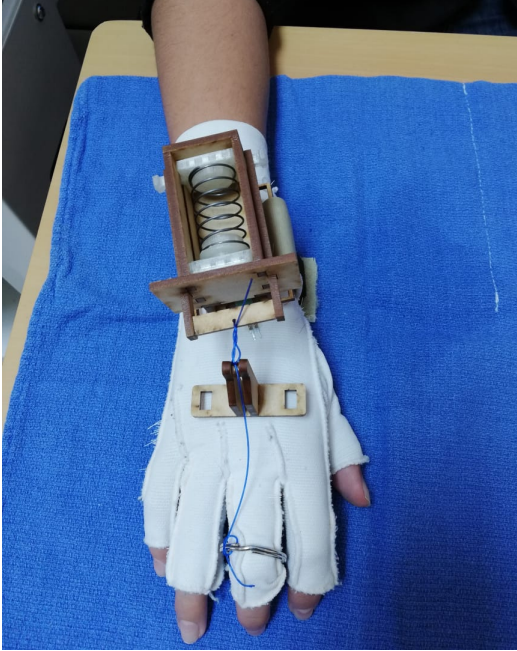
\includegraphics[width=0.5\linewidth]{img/TesisGuatemala.png}
        \caption{Prototipo dinamómetro Luis Carlos Ralon. Fuente Universidad del Valle de Guatemala }
        \label{fig:Prototipo dinamómetro Luis}
    \end{figure}    
\end{itemize}
\include{./tex/4_DicusiónClinica}
\capitulo{4}{Metodología}
En este capítulo voy a desarrollar los datos, las técnicas y métodos utilizados durante el proyecto. 
\section{Descripción de los Datos}
Para la realización del proyecto, no se han utilizado datos predefinidos por bases de datos, APIs públicas u otras fuentes de información.Los datos que aparecen son los obtenidos por los sensores durante las pruebas del dispositivo.
\section{Técnicas metodológicas de programación}
En esta sección se detallan las técnicas metodológicas de programación empleadas en el desarrollo del proyecto. 
\subsection{Lenguajes de programación}
En el proyecto empleé los siguientes lenguajes de programación especialmente seleccionados para cumplir con los requisitos de este.
\subsubsection{\textit{C++}}
Lenguaje de programación compilado y multiparadigma, caracterizado por su enfoque imperativo y orientado a objetos. Además, incluye el uso de programación general y funcional.
Muy utilizado en la creación de programas para la creación de interfaces y videojuegos.\cite{C++}\footnote{Pagina web con información de C++\cite{C++}.}

Se ha utilizado este lenguaje para la implementación de toda la lógica asociada a la placa Elegoo.
\subsubsection{\textit{Python}}
Python es un lenguaje alto de programación altamente usado, interpretado y multiplataforma. Diseñado para ser fácil de leer y escribir.
Ampliamente utilizado en el desarrollo web, ciberseguridad, aprendizaje automático, desarrollo de aplicaciones o la automatización de tareas, entre muchas otras aplicaciones.\cite{Python}\footnote{Pagina web con información de Python\cite{Python}.}
\subsubsection{\textit{Bash}}
Bash es un lenguaje de comandos y shell de Unix/Linux, también conocido como shell scripting o comandos de terminal.
Se ejecuta en una terminal o ventana de texto.\cite{Bash}\footnote{Pagina web con información de Bash\cite{Bash}.}

En este proyecto ha sido utilizado en la terminal de Rstudio para la creación de archivos, actualización de GitHub entre otras tareas.
----
\subsection{Bibliotecas}
La bibliotecas o librerías son un conjunto de funciones, clases y recursos ya escritos que se pueden utilizar de manera libre para agilizar procesos. 

\subsubsection{json}
Librería que permite la edición y adicción de documentos JSON.
\subsubsection{os}
Librería que permite la interacción con el sistema operativo.
\subsubsection{pandas}
Librería que permite el análisis y manipulación de datos.
\subsubsection{openpyxl}
Librería que permite leer, modificar y escribir archivos excel.
\subsubsection{Kivy}
Librería que permite la creación de interfaces gráficas de usuario(GUI).\cite{kivy}\footnote{Pagina web con información de kivy y documentación\cite{kivy}.}
\section{Entornos y aplicaciones}
En esta sección voy a realizar una recopilación de aplicaciones y entornos que he utilizado para la realización del proyecto, todas ellas explicadas y utilizadas en diferentes asignaturas del grado.
\subsection{Overleaf}
Herramienta en línea que permite redactar,editar,exportar y compartir con otros usuarios documentos científicos en formato LaTeX.

En este proyecto, se utiliza Overleaf para la creación de este documento y el anexo.
\subsection{RStudio}
RStudio es un entorno de software libre para computación estadística y gráficos. Tiene la capacidad de ejecutarse y compilarse en una amplia variedad de plataformas como Linux,MAC y Windows.\cite{Rstudio}\footnote{Pagina web con información de Rstudio\cite{Rstudio}.}

En este proyecto, se utiliza RStudio para realizar una unión entre el repositorio de GitHub y la carpeta de mi escritorio del ordenador donde voy avanzando el proyecto.
\subsection{GitHub}
GitHub es una plataforma basada en la nube cuya finalidad es almacenar,compartir y trabajar en conjunto con otros usuarios. 
Además, permite tener un seguimiento del trabajo, lo que permite ver todas las versiones que se van realizando de este mismo.\cite{GitHub}\footnote{Pagina web de GitHub\cite{GitHub}.} 

En este proyecto, GitHub se ha utilizado para realizar un seguimiento del proyecto, permitiendo que tanto el tutor como los miembros del tribunal puedan visualizar los cambios realizados y participar activamente en el proceso.
\subsection{Tinkercad}
Tinkercad es una aplicación web que permite la realización de diseños en 3D, la realización de circuitos y la posibilidad de escribir programas para dar vida a los diseños mediante la codificación.

En este proyecto, ha sido utilizada para la realización de la simulación del diseño del circuito electrónico, ya que permite utilizar diseños electrónicos ya hechos, modificarlos, añadir más componentes o empezar desde 0 un circuito.
\subsection{Visual Studio Code}
Visual Studio Code es una aplicación que funciona como editor de código fuente, personalizable y multiplataforma.
Permite al usuario la creación y edición de archivos en múltiples lenguajes y formatos, desde texto plano hasta YAML, pasando por JSON, Markdown, XML y muchos otros; además, gracias a sus múltiples extensiones, permite, entre otras cosas, el control de versiones con la extensión de GitHub o incluso el uso de IA con la extensión de Copilot.

En este proyecto, ha sido utilizada para realizar la interfaz y establecer la comunicación con la placa Elegoo, la elección de este editor se debió a las características mencionadas anteriormente, la facilidad de uso y la versatilidad, permitiendo un desarrollo ágil y eficiente del proyecto.
\subsection{Freecad}
Freecad es una aplicación multiplataforma, de código abierto y completamente gratuita, que permite al usuario crear diseños en tres dimensiones.
Es un modelador 3D paramétrico de código abierto, permitiendo así diseños lo mas proximos a la realidad.

En este proyecto, ha sido utilizada para realizar un modelo 3D para el proyecto.\cite{freecad}\footnote{Pagina web con información y posibilidad de descarga de freecad\cite{freecad}.} 

\section{Herramientas}
En esta sección voy a exponer y explicar las herramientas que he utilizado en el proyecto.
\subsection{Placa de Elegoo uno R3}
Placa de Arduino es una placa de desarrollo de código abierto. 
Integra el microcontrolador chip Atmel ATMEGA+328P principal y un ATmega16U2 para la comunicación con USB. \cite{Elegoo}\footnote{Pagina web con información de placa Elegoo\cite{Elegoo}.}

Esta formado con 14 pines digitales, 6 pines analógicos, 5 pines de energía, un puerto de USB para la conexión con el ordenador, un conector para la alimentación, un botón de reinicio,un resonador de cerámica de 16 MHz, leds indicadores y los puertos I2C y SPI.\cite{Arduino}\footnote{Pagina web con información de Arduino\cite{Arduino}.}
En la \textit{Figura \ref{fig:Placa Elegoo}} se puede ver una imagen del componente.
\begin{figure}[h]
        \centering
        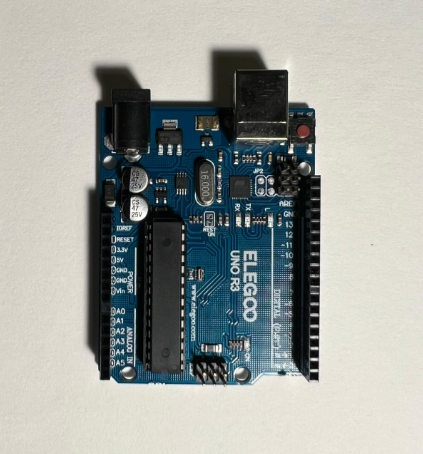
\includegraphics[angle=90,width=0.6\textwidth]{img/placa elegoo.png}
        \caption{Placa Elegoo}
        \label{fig:Placa Elegoo}
    \end{figure}

\subsection{Cables Dupont}
Alambres de metal conductor recubiertos de un plástico aislante flexibles que permiten las conexiones entre los propios componentes de la protoboard o entre la protoboard y la placa de Elegoo. En la \textit{Figura \ref{fig:cable_dupont}} se puede ver una imagen del componente.
\begin{figure}[h]
        \centering
        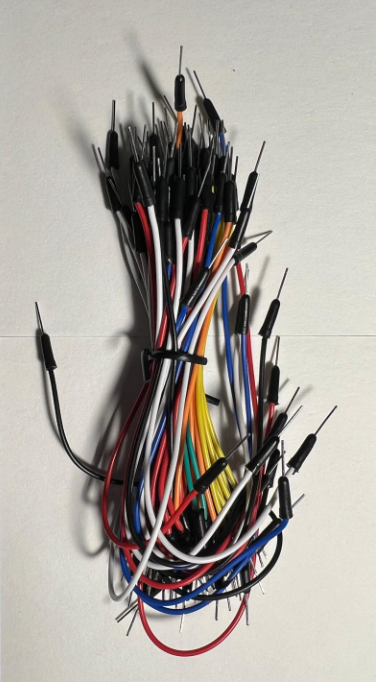
\includegraphics[angle=90,width=0.6\textwidth]{img/cable_dupont.png}
        \caption{Cables}
        \label{fig:cable_dupont}
    \end{figure}
   
\subsection{Cable USB}
Conector que une la placa Elegoo con el ordenador, permite introducir las instrucciones programadas en el ordenador en placa Elegoo. En la \textit{Figura \ref{fig:Cable USB}} se puede ver una imagen del componente.
\begin{figure}[h]
        \centering
        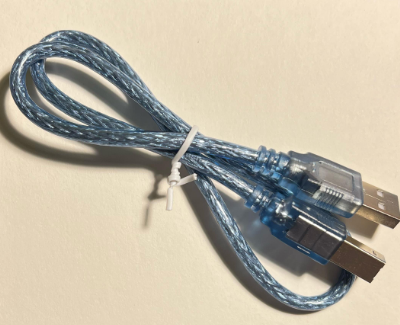
\includegraphics[width=0.5\textwidth]{img/cable usb.png}
        \caption{Cable USB}
        \label{fig:Cable USB}
    \end{figure}
   
\subsection{Resistencias}
Componentes electrónicos que limitan el flujo de la energía eléctrica en el circuito, son una medida de la oposición al flujo de corriente.  En la \textit{Figura \ref{fig:Resistencias}} se puede ver una imagen del componente.\cite{Resistencia}\footnote{Pagina web con información de las resistencias\cite{Resistencia}.}
\begin{figure}[h]
        \centering
        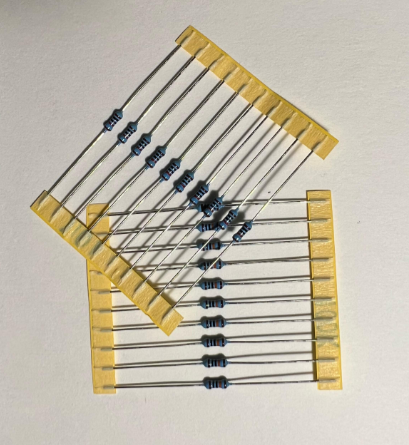
\includegraphics[width=0.5\textwidth]{img/Resistencias.png}
        \caption{Resistencia}
        \label{fig:Resistencias}
    \end{figure}
    
\subsection{Protoboard}
También llamada placa de pruebas, permite la creación de circuitos electrónicos.Es una matriz con orificios interconectados que permiten la inserción de componentes eléctricos. En la \textit{Figura \ref{fig:Protoboard} } se puede ver una imagen del componente.
\begin{figure}[h]
        \centering
        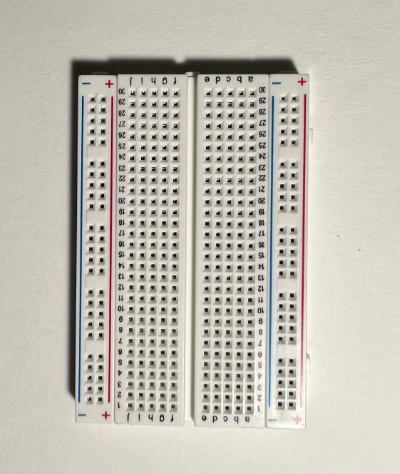
\includegraphics[angle=90,width=0.5\textwidth]{img/Protoboard.png}
        \caption{Protoboard}
        \label{fig:Protoboard}
    \end{figure}
\subsection{Posibles sensores}
En esta subsección se presentarán los sensores investigados para la realización del proyecto, el sensor seleccionado y el porqué de su selección.
\subsubsection{\textit{{Sensor fuerza resistivo}}}
Los sensores de fuerza resistivos son sensores capaces de detectar la presión o fuerza que se les ejerce.
Como su propio nombre dice, necesita para su uso una resistencia, la cual actúa como divisor de voltaje.
\subsubsection{\textit{{Células de carga}}}
Las células de carga son herramientas muy utilizadas en la industria para las mediciones de fuerza,compresión y tensión.
Son un tipo de transductores que convierten la fuerza aplicada  en una señal eléctrica medible. \cite{Celula_Carga}\footnote{Pagina web con información sobre las celulas de carga\cite{Celula_Carga}.}
Existen múltiples tipos de los cuales destacamos los siguientes:
    \begin{itemize}
        \item Células de cargas mecánicas: miden la fuerza mecánica al aplicarle un objeto, miden pesos.
        \item Células de carga extensométricas: miden deformaciones locales según su posición.La medida de la fuerza es determinada por la integración de los valores de cada valor individual, formado por un transductor de fuerza y un elemento elástico.\cite{celulas_extensométricas}\footnote{Pagina web con información de las células de carga de tipo extensométricas\cite{celulas_extensométricas}.}
        \item Células de carga hidráulicas:dispositivo llenó de un líquido con tiene una presión de precarga, al aplicar la fuerza aumenta la presión del líquido que es medida por un transductor de presión.
        \cite{Celulas_hidraulicas}\footnote{Pagina web con información de las células de carga de tipo hidraulicas\cite{Celulas_hidraulicas}.}
        \item Células de carga piezoélectricas: miden fuerzas dinámicas o cuasistáticas, tanto de tracción como compresión.Muy sensibles y rápidas.
        \cite{Celulas_piezoelectricas}\footnote{Pagina web con información de las células de carga de tipo piezoélectricas \cite{Celulas_piezoelectricas}.}
    \end{itemize}
En la \textit{tabla \ref{tab:comparacion_sensores}} se realiza un resumen donde se expondrán el tipo, características y precio aproximado de cada una de ellas.
\begin{table}[j]
\centering
\begin{tabular}{|l|p{8cm}|c|}
\rowcolor[HTML]{BFBFBF} 
\hline
\textbf{Tipo} & \textbf{Características de medición} & \textbf{Precio} \\
\hline
Células de carga mecánica & Rango de medición limitado, respuesta lenta, bajo costo, bajo mantenimiento & 10-200€ \\
\hline
Células de carga extensiométricas & Rango amplio (hasta 50 kN o más), buena precisión, alta estabilidad & 30-200€ \\
\hline
Células de carga hidráulicas & Medición de fuerzas grandes (hasta 100 kN), sin electrónica, resistente a ambientes hostiles & 50-300€ \\
\hline
Células de carga piezoeléctrica & Aproximadamente de 10 N a 300 kN, de precisión muy alta, ideal para fuerzas dinámicas & 60-500€ \\
\hline
Sensor de fuerza resistivo & Aproximadamente de 0-300N, precisión alta y de pequeño tamaño & 7-30€ \\
\hline
\end{tabular}
\caption{Tabla de comparación de sensores de fuerza}
\label{tab:comparacion_sensores}
\end{table}

Tras comparar los distintos sensores según su precio, características e integración, he concluido que los sensores de fuerza resistivos son la mejor opción para llevar a cabo el proyecto.

\subsection{{Sensor de fuerza resistivo}}
Como se ha explicado anteriormente los sensores de fuerza resistivos son sensores capaces de medir la fuerza ejercida con el uso de resistencias.

Para el proyecto se ha utilizado el sensor MD30-60 capaz de medir de 0 a 30Kg. 
\begin{figure}[h]
        \centering
        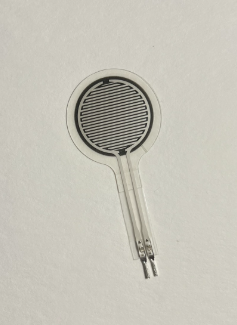
\includegraphics[,width=0.5\textwidth]{img/sensor.png}
        \caption{Sensor de fuerza MD30-60}
        \label{fig:Sensor de fuerza}
    \end{figure}
\capitulo{6}{Resultados}

\section{Resumen de resultados}

Se presenta en este capítulo un resumen de los resultados obtenidos durante el desarrollo del proyecto. 
\begin{itemize}
    
    \item \textbf{Elección de un sensor capaz de medir la fuerza ejercida por cada dedo.}
    
    Se ha utilizado el sensor de fuerza resistivo MD30-60, ofreciendo resultados satisfactorios en las pruebas realizadas. Con el objetivo de lograr un ajuste de las medidas lo más cercano a la realidad, se realizó una calibración en los sensores, para más detalle véase el Apendice G.1 del anexo. Además se realizó un análisis del porcentaje de error, ofreciendo como resultado, un valor de error medio de 4.6\%, con valores de pico de hasta un 10\% error.
    
    \item \textbf{Creación de un prototipo de dispositivo que pueda medir la presión ejercida por la mano.}
    
    Se ha logrado la creación de un prototipo funcional del dispositivo (\ref{fig:Prototipo Fisico}), cumpliendo con el diseño inicial de medir la presión ejercida por cada dedo de la mano de forma orientativa y repetible. Este prototipo integra cinco sensores de fuerza resistivos, una placa de arduino, una placa de pruebas, una luz led, un pin botón y otros materiales complementarios como resistencias y cables, proporcionando un prototipo integral que cumple con los requisitos necesarios. 

    Adicionalmente, se ha diseñado un accesorio complementario (\ref{fig:Accesorio}) que facilita el uso del dispositivo durante sesiones de rehabilitación. Tiene una dimensión de 60x60x135, con un agujero interior para insertar una de las barras de la
    tabla canadiense y cinco hendiduras destinadas a situar cada uno de los sensores.

    \begin{figure}
        \centering
        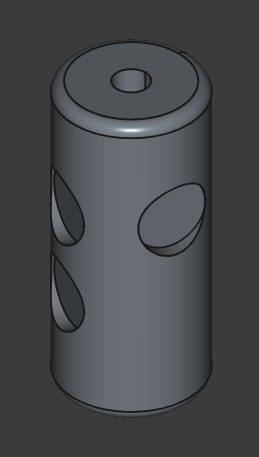
\includegraphics[width=0.25\linewidth]{img/Mango3.png}
        \caption{Accesorio para tabla canadiense. Fuente propia}
        \label{fig:Accesorio}
    \end{figure}
    \begin{figure}
        \centering
        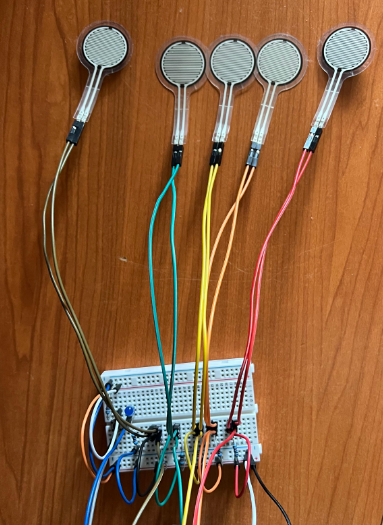
\includegraphics[angle=180,width=0.5\linewidth]{img/Prototipo_s.png}
        \caption{Prototipo físico. Fuente propia}
        \label{fig:Prototipo Fisico}
    \end{figure}
    \item \textbf{Seguimiento de evolución de los pacientes.}

    Se ha desarrollado un prototipo de interfaz tipo desplegable, capaz de almacenar los datos obtenidos por los sensores en un archivo xlsx. Además de su almacenamiento, permite al profesional la visualización de estos mediante una tabla (\ref{fig:tabla-registro}) o representando los datos mediante una gráfica (\ref{fig:Grafica-datos}). 
    
    La estructura y visualización de los datos recolectados se amplía en el Apéndice D del anexo.
    \begin{figure}
        \centering
        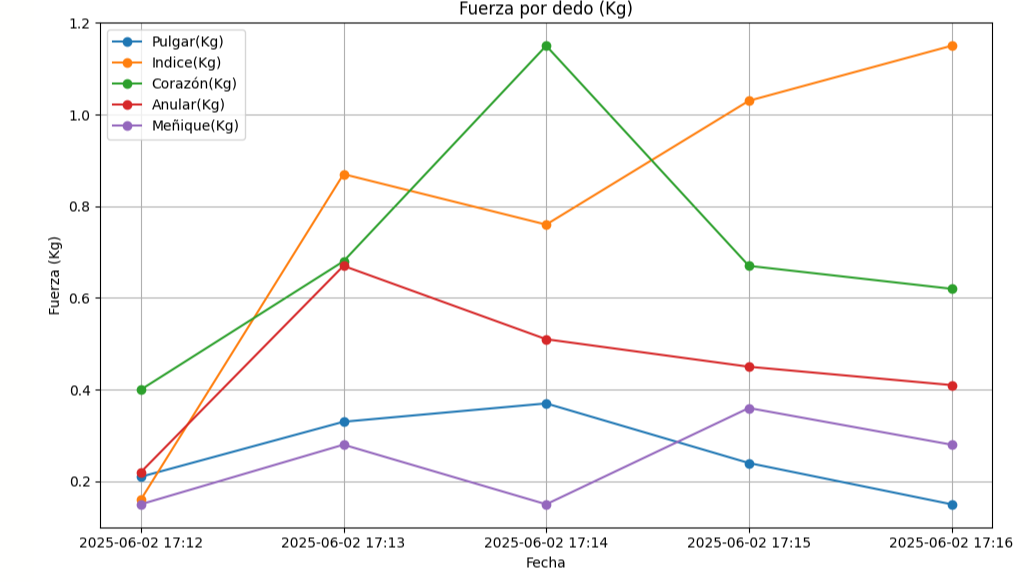
\includegraphics[width=0.8\linewidth]{img/grafica_fuerza.png}
        \caption{Representación datos en gráfica. Fuente propia}
        \label{fig:Grafica-datos}
    \end{figure}
    \begin{figure}
        \centering
        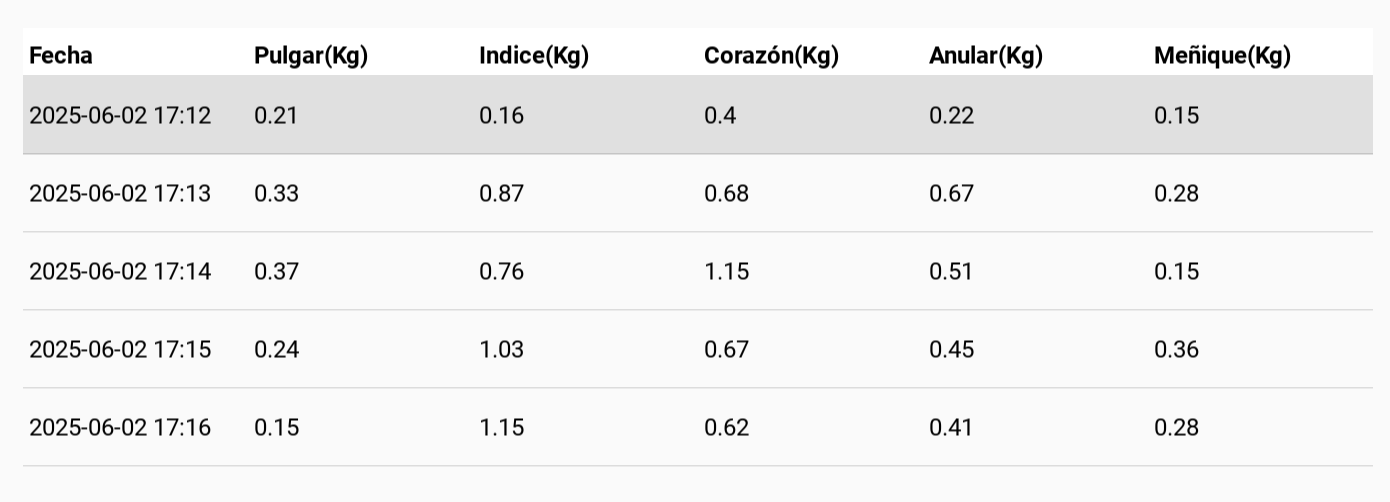
\includegraphics[width=1\linewidth]{img/Datos_medidas.png}
        \caption{Tabla de registros. Fuente propia}
        \label{fig:tabla-registro}
    \end{figure}
    \item \textbf{Comparativa de prototipos}
    
    Tras la realización del proyecto, he realizado una comparativa con otros prototipos mencionados en la sección 'Estado del arte'.

    A pesar de que los 3 prototipos emplean los sensores resistivos y tienen como finalidad el seguimiento de los pacientes para facilitar la recuperación, existen algunas diferencias. 
    En la tabla \ref{tab:comparacion_diseños} se presenta una comparativa de los 3 dispositivos.
\end{itemize}


\begin{table}[h]
    \centering
    \begin{tabular}{|p{2.5cm}|p{3.5cm}|p{4cm}|p{3.8cm}|}
    \rowcolor[HTML]{BFBFBF} 
    \hline
    \textbf{Aspecto} & \textbf{Juliana Gómez et al.} & \textbf{Luis Carlos Ralón Gordill} & \textbf{Diseño propio} \\ \hline
    Sensor utilizado   & FSR  & FSR  & FSR \\ \hline
    Número de sensores   & 5  & 1  & 5 \\ \hline
    Uso del resorte & Transmisión de fuerza & Generar resistencia  & No aplica   \\ \hline
    Mecanismo de transmisión   & Mediante resorte  & Mediante resorte & Directo  \\ \hline
    Ventajas   & Alta precisión  & Uso en niños  & Uso aplicabilidad múltiple \\ \hline
    Limitaciones & Solo permite el agarre de precisión & Fallos en Resorte-Sensor & Error medio de 4.6\% \\ \hline
    Visualización & Interfaz, visualización en el momento & Interfaz gráfica, visualización en el momento& Interfaz desplegable, con posibilidad de ver registros anteriores \\ \hline
    Coste    & No menciona    & No menciona precio exacto, pero deja claro que busca producir el menos coste y al utilizar un único sensor el coste total es bajo. & 78€ \\ \hline
    \end{tabular}
    \caption{Comparación de los prototipos.}
    \label{tab:comparacion_diseños}
\end{table}
    
\section{Discusión}

Los resultados obtenidos cumplen con los objetivos marcados en el inicio del proyecto. Se ha logrado realizar un prototipo de interfaz y dispositivo capaz de registrar los datos recogidos por los sensores.

La implementación de los gráficos en la visualización de los registros permite una representación clara de la evolución de los pacientes durante las sesiones. Facilitando la interpretación de los datos recogidos por los profesionales sanitarios, detectando progresos, fatiga muscular o estancamientos, factores muy útiles en la toma de decisiones médicas.

Además, la protección de los datos es uno de los aspectos fundamentales en la creación del dispositivo. Se cumplen en todo momento mediante la encriptación de los documentos. El uso de bibliotecas para el cifrado se detalla en el Apéndice C.1 y D.1 del anexo.

Por último, destacar la utilización de materiales que impliquen el menor coste posible en la realización del dispositivo. El análisis económico detallado y la viabilidad legal se exponen en los Apéndices A.3 y A.4 del anexo.
\capitulo{7}{Conclusiones}

Concluido el desarrollo integral del proyecto, se presentan las principales conclusiones obtenidas del trabajo realizado:

\begin{itemize}
    \item El sensor de fuerza resistivo seleccionado cumple con los requisitos esperables, siendo favorable su utilización como método de cuantificación, con un promedio de error de 4.6\%.
    \item El diseño de los prototipos, tanto físico como de software, cumplen con los requisitos planteados. 
    \item Actualmente, no existe un dispositivo de bajo coste en el mercado que realice esta tarea, por lo que mejorar el diseño propuesto puede abrir una oportunidad dentro del mercado tecnológico-sanitario.
\end{itemize}
\capitulo{8}{Líneas Futuras}
Al tratarse de un prototipo, se pueden realizar varias mejoras para llegar a un dispositivo comerciable, robusto y de bajo coste.

Una de las primeras mejoras que podría implementarse es la eliminación del botón físico del dispositivo destinado a inicio de la medición, de manera que esta se active directamente al presionar 'Iniciar medición' en la interfaz. 

Asimismo, se podrían diseñar diferentes tipos de mangos donde poner los sensores, variando tanto en tamaño como en los materiales a utilizar. Debido a que el medio utilizado es impresión 3D, las posibilidades de personalización son muy amplias. Se podría utilizar material semielástico, permitiendo así una leve deformación, ya que estos materiales combinan flexibilidad y resistencia. Otra posibilidad, podría ser emplear compuestos como mezclas de PLA con polvo metálico, que aportarían mayor rigidez y peso, lo que supondría un desafío adicional durante el ejercicio.

De otra manera, se puede emplear un cambio en el tamaño ajustando el diámetro del mango. Contar con estos diferentes diámetros facilita el agarre para las personas según las diferentes patologías que tengan ya sea que afecten la movilidad o fuerza de la mano.

Además, se podría implementar una funcionalidad que permita generar un informe final por paciente imprimible, permitiendo que forme parte de la historia clínica. Usando la biblioteca FPDF, podemos generar archivos pdf con posibilidad de imprimir.

Por último, mejorar el desplegable para que se abra como una aplicación más de escritorio y no haga falta acceder desde el CMD o terceras aplicaciones como Visual Studio Code.
Con Kivymd solo se podrá realizar esto para archivos con sistema operativo Windows, para realizarlo se deberá crear un paquete especial siguiendo los pasos de la documentación de Kivymd \cite{kivymdapp}.

\bibliographystyle{apalike}
\bibliography{bibliografia}

\end{document}